\chapter{Anomalies}
\label{chp:anomalies}


This thesis will propose the SpreadRank algorithm,
 which will detect traffic spreading on OSI layer 4.
What this means, is that it will detect end-hosts (clients and servers) that initiate the same kind of connections that they receive.
The discriminator used to identify same-kind connections is the \gls{contact port} number associated with a flow.
The assumption is that a service both receiving and initiating connections to the same port is an anomaly.
For example, a workstation with a web browser and e-mail client will initiate connections to ports 80 (HTTP), 443 (HTTPS), 587 (SMTP submission) and 143 or 993 (IMAP and IMAPS respectively).
However, it is not expected that such a workstation would \emph{receive} connections towards these port numbers.
Neither is it expected that the web server would initiate connections directed towards port 80 or 443.

This is not true for all protocols.
For example, a mail server can forward e-mail to another mail server via port 25 (SMTP),
 and this second mail server may forward it to a third mail server over port 25 and so forth.
There are several other protocols that exhibit natural spreading, these are described in section~\ref{sec:proto_spreading}.



\section{Servers undergoing maintenance}
\begin{figure}[h!]
	\caption{Observed spreading caused by a server under maintenance}
	\label{fig:spread_maintenance}
	\centering
		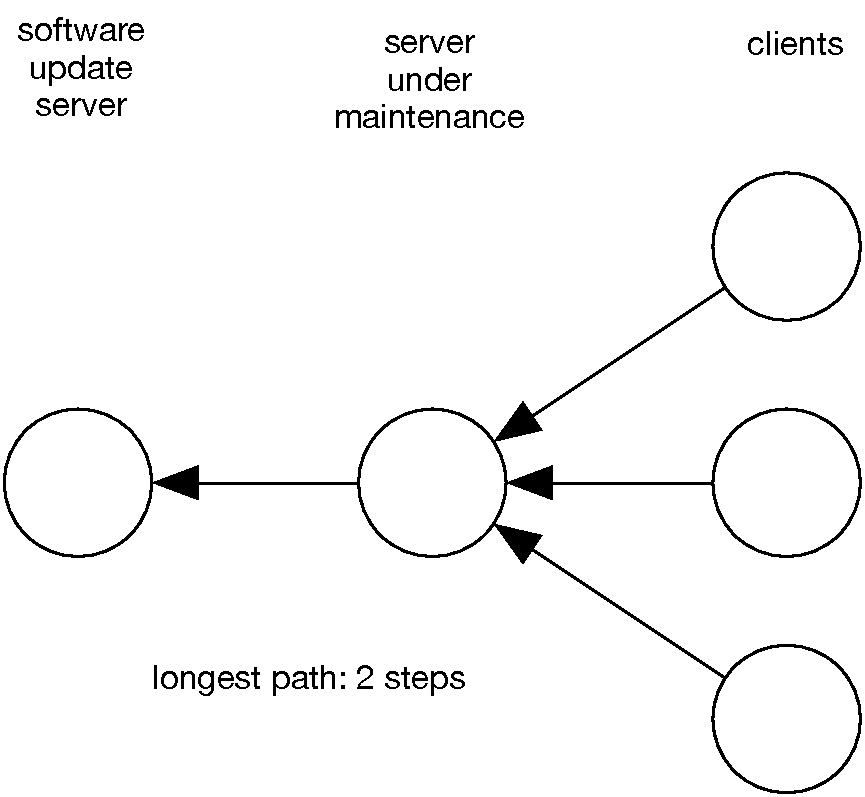
\includegraphics[width=0.5\textwidth]{spread_maintenance}
\end{figure}
Figure~\ref{fig:spread_maintenance} shows spreading caused by a server undergoing maintenance.
A server undergoing maintenance may connect to another server,
 for example to get the latest software updates.
Additionally, there exists server software that includes a graphical user interface,
 which gives the server the same look and feel as a workstation.
On these servers, the administrator may be inclined to use a web browser to download software or even browse the web.


\section{Home connections which run a personal server}
\begin{figure}[h!]
	\caption{Observed spreading caused by a single home server}
	\label{fig:spread_home}
	\centering
		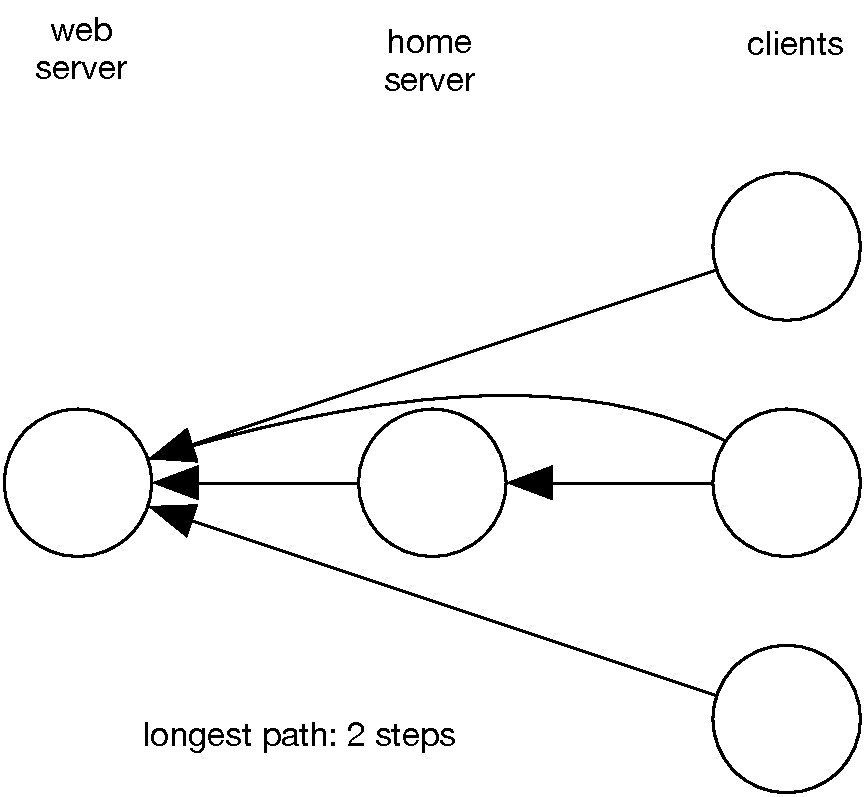
\includegraphics[width=0.5\textwidth]{spread_home}
\end{figure}

Figure~\ref{fig:spread_home} shows spreading caused by servers run by home users on a shared public IP address.
Users with a home server will often run the home server on the same IP address as the client.
This is done either by simply using the same machine as server and client,
 or by using a NAT router, allowing a separate client and server machine to share a public IP address.
When a client and a server share an IP address, this IP address will generally both receive and initiate flows.
Since there is no direct way to distinguish whether incoming and outgoing flows are related,
 such a situation might register as a case of spreading.
However, home servers are quite common, but a trail of home users with servers contacting each other can show up as an anomaly.


\section{VPN servers}
\begin{figure}[h!]
	\caption{Observed spreading caused by a VPN server}
	\label{fig:spread_vpn}
	\centering
		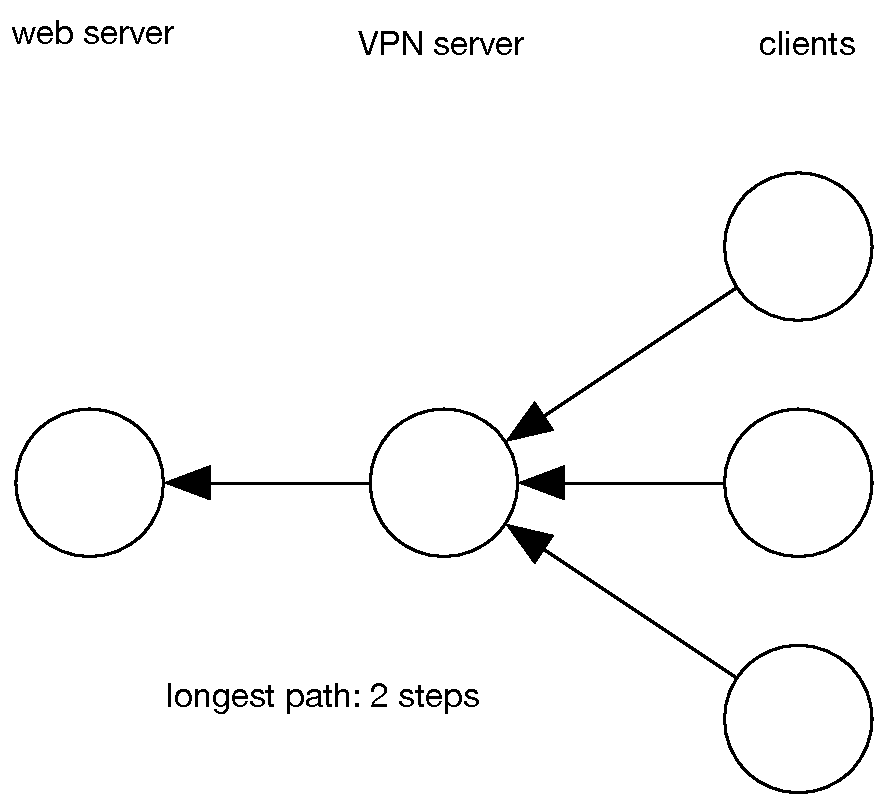
\includegraphics[width=0.5\textwidth]{spread_vpn}
\end{figure}

Clients can set up a secure connection to a VPN server (figure~\ref{fig:spread_vpn}).
All internet traffic initiated at the client (apart from the VPN traffic itself) will be sent to the VPN server in encapsulated form.
The VPN server removes the encapsulating, and forwards the traffic towards the internet, possibly mimicking a client.
Thus, if the client tunnels another VPN connection through the VPN server, the VPN server may appear to be a VPN client as well.

Some providers allow using SSH, HTTP or HTTPS for VPN.
Examples of software that can do this are sshttp~\cite{github:stealth:sshttp} and Microsoft RRAS~\cite{rras}.
When a user connects to a VPN server over HTTPS, and then uses the VPN to connect to a HTTPS host, this can register as spreading.
However, some VPN servers allocate dedicated public IP addresses to their clients,
 which means that connections are not forwarded over the same IP, which means that the VPN does not register as spreading.


\section{Protocols with natural spreading}
\label{sec:proto_spreading}
\subsection{BGP}
BGP is a protocol used by routers to exchange routing information.
Even though routers are level three devices themselves, they exchange routing information with each other the same way end-hosts do.
Routers both listen for incoming BGP connections, and send BGP to neighbouring routers at regular intervals.
Since routers both receive and initiate BGP flows, BGP spreading is expected to be high.

\subsection{DNS}
Clients use DNS to find the IP address associated to a hostname.
If the DNS server does not have the record in its cache,
 it must forward the query to an upstream server,
 or find the authoritative DNS server for that host and forward the query there.
Forwarding DNS is expected to cause high spreading.


\subsection{SMTP}
Most e-mail clients are configured with a so-called ``smart host'',
 which is the server that all outgoing mail is sent to.
This smart host will then find out which server handles e-mail for the recipient, and forward the message there.
In some cases, the e-mail will pass multiple servers before finally reaching a mailbox.
Naturally, this means that some spreading in the SMTP protocol is expected.


\section{HTTP/HTTPS}
\label{sec:http}
A large number of different services use HTTP and HTTPS as underlying layer for their data.
SpreadRank may therefore observe trails of machines connecting over port 80 or 443,
 without these flows actually being related.
There is currently no direct way to view the difference between different services provided over HTTP or HTTPS, purely based on NetFlow data.

%Possibly less clear cases of spreading are \gls{SSH} and \gls{HTTP}.
%Although these protocols are meant for client-server communication (\gls{SSH} allows clients to connect to a remote shell, \gls{HTTP} is the protocol used for web pages),
% it is possible that a user will use the SSH session to another SSH server from there.
%A proxy web server can request a page on its clients behalf.
%These services yield low depths, as most servers providing these services will not forward information they receive.


\section{Combination}
\begin{figure}[h!]
	\caption{Observed spreading caused by a combination of benign factors}
	\label{fig:spread_combi}
	\centering
		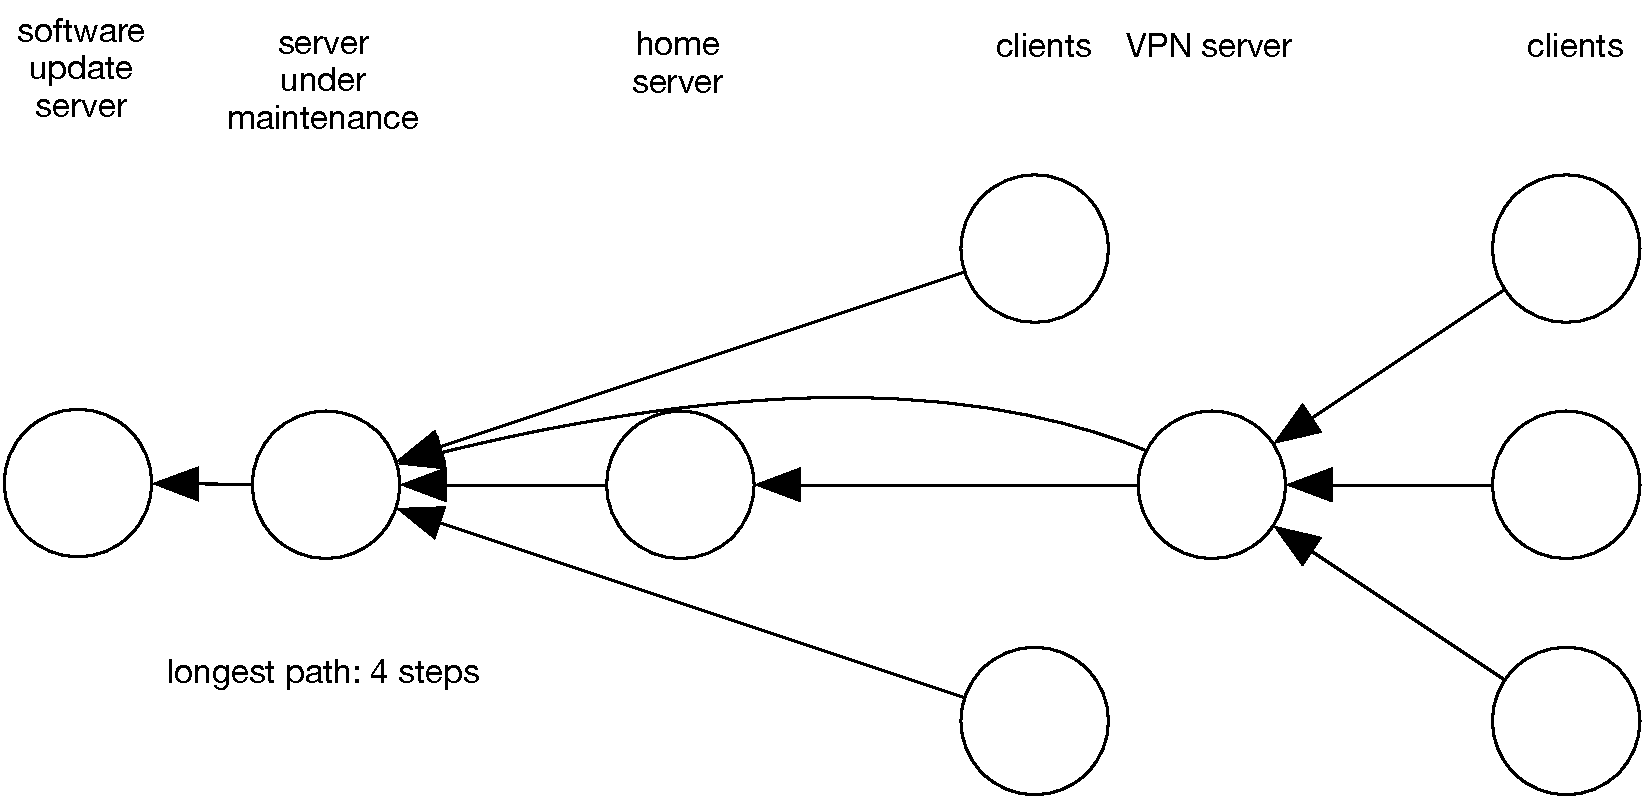
\includegraphics[width=0.75\textwidth]{spread_combi}
\end{figure}

A combination of different occurrences of spreading may lead to larger spreading, as shown in figure~\ref{fig:spread_combi}.
However, the depth, is still relatively limited.
This means that relatively short paths are not anomalies.
%From which length spreading becomes an anomaly depends on the protocol and the size of the NetFlow dataset,
% but from the results of the experiment, 20-30 steps seem like a reasonable amount.
%Because of this, if only a single host is observed generating the same kind of traffic as it receives, no conclusions can be drawn from that.
%However, if there is a long trail of hosts sending the same kind of traffic, there is a good chance that this is a worm at work.


\section{Worm infection}
A worm is a piece of software that is programmed to infect other hosts in such a way that these hosts will run the worm, too.
It infects a host by looking for systems that run unpatched software,
 and using a known security hole to get access to the service and install itself.
After infection, the victim will start doing the same.
This process can go on for ever, until a system administrator starts blocking these flows.
Consequently, a worm that successfully spreads over many end-hosts, will show large spreading.


\section{Peer to peer traffic}
Peer to peer traffic is another case of spreading that happens intentionally;
a hallmark example is BitTorrent.
BitTorrent is a protocol for distributed file sharing, where all clients will make chunks they have downloaded available to other clients.
This differs from the traditional client/server model, where clients do not spread information to other clients but get all their information from a central server.
BitTorrent, however, operates over many different port numbers, which makes it difficult to match incoming and outgoing flows together.

The same is true for Tor traffic.
Tor is a mechanism for anonymous internet access, which works by encrypting traffic and routing it at random through multiple hops,
before sending it to the final destination.
Tor also operates on random ports, which makes it difficult to match flows together.

\subsection{Stealth worm}
Due to BitTorrent and Tor being able to hide their activity from an algorithm as SpreadRank,
the question arises whether a worm can do the same thing to hide its activity.
The important difference between benign traffic, such as BitTorrent and Tor, and malicious traffic such as worms,
is consent from the owner of the host.
If a host is participating in BitTorrent or Tor, it is because the owner of the host voluntarily installed software to supports these protocols.
Because these protocols can rely on software being installed, they can use virtually any connection model imaginable.

This is different for malware;
the initial infection must happen through a known vulnerability in the host.
This vulnerability will typically be part of the operating system or some type software that is installed.
Malware has therefore limited possibilities for infection, and must follow the specification of the software it wants to attack, which will often run on a standard port.
Thus, in order to attack a specific service, malware must target the same port for every attack.

Once a host has been infected, the malware can install itself, and it may communicate with command-and-control servers through stealth communication channels that may not be as easy to detect.
However, it will in all likelihood still try to attack other hosts, to increase the amount of infected hosts, for which it will have to generate observable traffic, for reasons mentioned earlier.



